%% LyX 2.0.6 created this file.  For more info, see http://www.lyx.org/.
%% Do not edit unless you really know what you are doing.
\documentclass[12pt,english]{article}
\usepackage[T1]{fontenc}
\usepackage{geometry}
\geometry{verbose,tmargin=1in,bmargin=1in,lmargin=1in,rmargin=1in}
\usepackage{graphicx}
\usepackage{setspace}
\usepackage[authoryear]{natbib}
\doublespacing

\makeatletter
\@ifundefined{date}{}{\date{}}
%%%%%%%%%%%%%%%%%%%%%%%%%%%%%% User specified LaTeX commands.
\usepackage{longtable}
\usepackage{dcolumn}
\usepackage{pdflscape}
\usepackage{graphicx}
\usepackage{endnotes}
\usepackage{lscape}

\makeatother

\usepackage{babel}
\usepackage{xunicode}
\begin{document}
\begin{doublespace}

\title{\textbf{\large{Mass Media and the Domestic Politics of Globalization}}}
\end{doublespace}

\maketitle
Although the relationship between economic globalization and the modern
welfare state has been one of the most studied issues in political
economy over the past three decades (e.g., \citealt[316]{Gourevitch:1978bn,Garrett:1995tj,Rodrik:1998te,Burgoon:2001dp,Adsera:2002vt,Oatley:2011hv}),
recent research on public opinion and political behavior in open economies
raises serious questions about the assumptions of this tradition (\citealt[155]{Hellwig:2007wt}).
A fundamental assumption in globalization-welfare research, which
dates back to Karl Polanyi's \emph{The Great Transformation,} is that
policymakers who wish to liberalize economic markets are held accountable
by those groups who would suffer the adjustment costs (Polanyi {[}1944{]}
\citeyear[79, 385]{Polanyi:2001vc}). Scholars have shown that to
sustain political coalitions in favor of opening national economies,
national policymakers have to compensate protectionist domestic groups
with side payments in the form of social welfare programs (\citealt[1028-29]{Katzenstein:1985ub,Rodrik:1998te,Adsera:2002vt}).

However, research in comparative political behavior shows that as
domestic economies become increasingly integrated, citizens perceive
that governments have less ``room to maneuver'' and accordingly
shift their blame away from domestic policymakers to the unaccountable
pressures of the global economy (\citealt{Alcaniz:2010gb,Hellwig:2012vk}).
Citizens in countries highly exposed to the global economy are less
likely to punish incumbents for a poorly performing economy (\citealt{Hellwig:2007gn})
and more likely to base their vote on non-economic issues (\citealt{Hellwig:2008ia}).
If domestic groups do not punish politicians for economic losses made
possibile by the political decisions to maintain open national economies,
then an essential causal link in current accounts of the globalization-welfare
nexus may not hold under certain conditions. Furthermore, this current
of research has yet to take seriously that economic globalization
does not \emph{inherently} constrain policymakers' ``room to maneuver''
but rather has been socially constructed as such by elites and typically
through the mass media (\citealt{Hay:2011dh,Hay:2005dh,Hay:2002iy}).

At the same time, previous research has shown that mass media have
direct effects on perceptions relevant to how citizens are likely
to understand the politics of globalization. Specifically, mass media
have direct effects on perceptions of responsibility (\citealt{Iyengar:1987uo};
\citealt{Iyengar:1991uf}), the politicization of economic hardship
(\citealt{Mutz:1992ww}; \citealt{Mutz:1994kp}), and civic engagement
more broadly (\citealt{Putnam:1995vj}; \citealt{Norris:2000uf}).
In the specific context of the distributive domestic politics of globalization,
the preponderance of previous research strongly converges on a set
of counter-intuitive arguments: By amplifying the dominant construction
of globalization as an external imperative constraining policymakers
and in this way shifting citizen blame attributions away from governments
and toward international forces, the mass media should reduce the
ability of domestic groups to hold national policymakers accountable
for the effects of economic openness. In turn, as the global economy
and mass media penetrate states, national policymakers should face
less pressure to compensate protectionist domestic groups for economic
hardships linked to the global economy. As states become increasingly
penetrated by both the global economy and mass media, at the state-level
we should observe a weakened relationship between economic openness
and welfare spending.

These expectations are tested with survey data and state-level economic
data ideally suited to assess the implications of these arguments
at both levels of analysis. A Legidoscope survey from France in 1992-1993
provides a uniquely valuable opportunity to test the argument that
mass media has independent effects on individuals' perceptions, blame
attributions, and behavior around issues of economic openness. The
findings show that mass media exposure is positively associated with
individuals' perceptions of economic openness as a problem and then,
controlling for whether economic openness is perceived as a problem,
the attribution of blame to international forces. For comparability
with respect to previous research on the globalization-welfare nexus,
the state-level implications of the theory are tested on pooled cross-sectional,
time-series data from most countries in the world between 1960 and
2010. Using penetration rates of information-communication technology
(ICT) as a proxy for the prevalence of mass media within states---in
particular, the number of newspapers, televisions, and radios per
person---several analyses across multiple model specifications suggest
that the spread of ICT and the mass media they carry is associated
with a weakening of the positive relationship between economic openness
and social welfare spending. The dampening effect of mass media holds
after controlling for several rival explanations and when included
in the replication of previous, influential studies. Consistent with
the survey analysis, the state-level associations are interpreted
as evidence for the argument that policymakers are more likely to
neglect domestic groups harmed by political decisions to liberalize
markets the more prevalent is mass media within their states. Specifically,
this is because mass media tends to shift the perceptual and behavioral
response of protectionist individuals away from blaming and acting
against the government on the politics of openness.

These findings alter the prevailing wisdom in at least two ways. First,
they provide new evidence for the claim that economic openness makes
citizens less likely to blame, and less likely to punish, incumbent
governments for poor economic performance, but they also reveal that
mass media exposure may be an alternative and independent causal path
to the same effect, controlling for perceptions of economic openness.
Second, this is one of the first systematic investigations of mass
media as a political \emph{institution} that conditions the domestic
politics of the global economy. As such, it directly responds to calls
for more truly political accounts of the domestic effects of globalization
(\citealt[341]{Kayser:2007iga}) and for a more rigorous examination
of the micro-foundations of work in this tradition (\citealt{Hays:2005vo,Walter:2010ky}).

The article proceeds as follows. In the first section, previous literature
is reviewed to reveal a gap between comparative and international
political economists on the one hand and scholars of public opinion
and political behavior on the other, and to suggest how mass media
research speaks directly to this gap. A second section develops specific
hypotheses regarding how mass media is likely to affect individual
perceptions, blame attributions, and electoral accountability around
the politics of economic openness. A third section discusses the data
and modeling strategy, the penultimate section discusses the core
findings, and a final section concludes.


\section{{\normalsize{Mass Media Between Globalization and Domestic Politics}}}

One of the most robust findings in international and comparative political
economy is the positive state-level correlation between international
trade and size of the public sector (\citealt{Cameron:1978vb,Rodrik:1998te,Garrett:1995tj,Adsera:2002vt}).
Most political scientists theorize this regularity as \textquotedbl{}embedded
liberalism,'' exemplified in the postwar proliferation of Keynesian
social pacts that promoted open national markets with state-sponsored
social protections (\citealt{Ruggie:1982wx}). Although social scientists
widely agree that the expansion of international trade is welfare-improving
in the long run, they also agree that the construction or expansion
of markets often induces political backlash from domestic groups in
the short run. This backlash requires policymakers in favor of increasing
openness to compensate such groups through side payments, typically
in the form of redistributive social spending, lest the necessary
political support for increasing openness breaks down. Even across
much disagreement about which aspects of economic openness have the
most effect on the various components of welfare spending (\citealt{Mares:2004el,Ansell:2008wl,Burgoon:2001dp}),
in which countries the relationship holds (\citealt{Rudra:2002ui}),
and even whether the focus on economic openness per se is misspecified
(\citealt{Kim:2007wu,Oatley:2011hv}), scholars are generally in agreement
about the expectation that liberalization of national markets elicits
a corresponding political backlash from those domestic groups who
would bear the adjustment costs.

Despite the leverage it provides to models of the relationship between
globalization and welfare-state effort, there is surprisingly little
evidence for the assumption that domestic groups harmed by economic
liberalization exert sufficient political pressure on national policymakers
that policymakers provide welfare compensation to appease them. Hays,
Ehrlich, and Peinhardt \citeyearpar{Hays:2005vo} find evidence that
government spending helps sustain support for free trade, and Walter
(\citeyear{Walter:2010ky}) finds consistent evidence in Swiss survey
data for multiple points in the individual-level causal chain of the
compensation thesis. This current of research on the individual-level
evidence for a compensation dynamic does not, however, answer the
very different question of whether the economic insecurity induced
by globalization induces an electorally significant threat for liberalizing
policymakers. Margalit (\citeyear{Margalit:2011hm}) finds that job
losses due to offshoring had a stronger negative effect on incumbent
vote share than job losses not related to offshoring. Additionally,
that study also finds that spending from the Trade Adjustment Assistance
program significantly reduced the size of the effect. Still, it remains
unclear whether and how other institutions moderate the public perceptions
and electoral consequences of liberalization and if different dimensions
of liberalization have the same domestic effects as offshoring in
particular. For instance, \citet{Guisinger:2009vt} finds that trade
policy may not be sufficiently salient, even to the most affected
groups, to justify voter-driven models of trade policy. Baker (\citeyear{Baker:2003ci,Baker:2005jg,Baker:2009ta})
argues that, especially in the developing world, public support for
trade openness remains high because it is associated with relatively
high-quality goods at relatively low prices, despite sometimes dramatic
negative macro-economic consequences. Such findings from Guisinger
and Baker highlight pathways through which certain negative effects
of trade liberalization can have different effects on individuals,
depending on how they are perceived. Baker's finding of high support
for free trade even in national contexts of dramatic negative macro-economic
consequences, only adds scholarly interest to the puzzle of precisely\emph{
how} and \emph{why} individuals come to find consumption effects more
salient than other effects of trade liberalization.

Other research also suggests causal pathways through which citizens
harmed by the adjustment costs of liberalization would not hold policymakers
accountable for the political decision of liberalization. First, research
mostly from advanced democratic countries finds that as the sources
of economic growth shift, citizens accordingly adjust their expectations
of government policymaking and their attributions of blame for national
problems.%
\footnote{Expectations of government policymaking and blame attributions are
not only driven by material or institutional changes in the political
economy but may also be endogenous to vote choice or the partisan
composition of an incumbent government (\citealt{Wlezien:1997ia}).%
} Using time-series data from France between 1985 and 2002, Hellwig
shows that as exposure to trade and capital flows increase, citizens
becomes less confident in the ability of national policymakers to
solve national problems and the public demand for economic policy
solutions decreases (\citealt{Hellwig:2007wt}). Voters also adjust
their judgement of governments in predictable ways as other components
of the institutional context change. For instance, when the Bank of
England gained political independence, British voters were less likely
to base their evaluation of the government on monetary policy and
more likely to base it on fiscal policy (\citealt{:2010fv}). Just
as evaluations of government shift with the material and institutional
sources of economic outcomes, so too does blame for national economic
problems.

Secondly, perceptions and blame attributions affect political outcomes
by altering what policymakers can be credibly held accountable for.
Analyzing all 560 democratic elections between 1975 and 2002, Hellwig
and Samuels (\citeyear{Hellwig:2007gn}) show that as trade and capital
flows increase as a share of gross domestic product, domestic economic
growth rates have a smaller effect on incumbent vote share. Cross-sectional
analyses of French and British survey data from 1997 and 2001, respectively,
show similar effects of globalization on the determinants of vote
choice, decreasing the effect of voter's economic performance evaluations
and party positions on economic issues (\citealt{Hellwig:2008ia}).
Perceptual shifts in the ability of governments to affect economic
policy also affect voter turnout. Analysis from the United States
has found that individuals who suffer the economic adversity but do
not blame the government are less likely to vote than comparable individuals
who do blame the government (\citealt{Arcenaux:2003ue}). In terms
of policymaking, elite messaging in the mass media (\citealt{Hellwig:2011iu})
and interviews with party elites in Europe (\citealt[206]{Hellwig:2012vk})
confirm that politicians consciously stress globalization constraints
on their own behavior. Additionally, changes in the institutional
setting are found to have predictable moderating effects on the responsivness
of policy to public opinion. For instance, Sattler, Brandt, and Freeman
(\citeyear{:2010fv}) show that before central bank independence,
British fiscal and monetary policies were responsive to aggregate
voting intentions and government approval ratings but, after central
bank indepedence, monetary policy was no longer responsive. Interestingly,
however, Sattler, Brandt, and Freeman \citeyearpar{Sattler:2008vw}
find mutual responsiveness between public opinion and policy \emph{outputs},
despite a lack of responsiveness in policy \emph{outcomes} such as
inflation and economic growth. That this responsiveness is observed
outside real economic outcomes is accredited to the difficulty of
identifying the effects of policies in open economies.

Given that public perceptions of the institutional context have been
shown to affect political consequences of the economy, it is puzzling
that scholarship on the domestic politics of economic globalization
has largely neglected a serious inquiry into political communication
and the mass media in particular. Scholars of American politics have
shown that national policymakers actively engage in strategies of
``blame avoidance'' through the mass media (\citealt{Weaver:1986ku,Jacobson:1983tg}),
diffusing blame horizontally toward other equals or vertically upward
in the chain of authority (\citealt{McGraw:1990kk,McGraw:1991up}).%
\footnote{\citet[20]{Hood:2002ko} suggests that by lowering the potential costs
of communicating malign policy effects to harmed groups, mass media
may increase the incentives for politicians to avoid blame. See also
\citet{Hood:2009ed}.%
} Variation in blame attributions, in turn, has predictable effects
on how individuals judge both policies and policymakers (\citealt{McGraw:1995up}).
Other work has shown that under certain conditions mass media can
diffuse blame through issue framing (\citealt{Iyengar:1987uo}; \citealt{Iyengar:1991uf}),
depoliticize personal experience in favor of sociotropic perceptions
(\citealt{Mutz:1992ww}), and exacerbate inequalities in political
participation (\citealt{Norris:2000uf}). More generally, a formidable
and highly critical tradition of observers have advanced richly argued
but largely untested propositions converging on the expectation of
profoundly antidemocratic tendencies in the modern mass media (\citealt{Herman:1988ta,adorno2001culture}).
In light of these currents, it is a surprising omission in previous
research on the domestic politics of globalization that testimony
by party elites in research interviews (\citealt[206-07]{Hellwig:2012vk})
and via the mass media (\citealt[420-21]{Hellwig:2011iu}) is more
often cited as evidence of room-to-maneuver constraints than questioned
as possible strategic communication or media bias. Especially because
evidence for opinion-policy responsiveness in open economies can be
observed apart from and despite the objective economic effects of
policy \citep{Sattler:2008vw}, a necessary next step in studying
the domestic politics of globalization is to theorize more specifically
how political communication---in particular, the mass media---directly
and indirectly affects the relationship between objective patterns
of economic openness and domestic political outcomes.


\section{{\normalsize{Theory and Hypotheses}}}

A central premise of this article is that issues of economic openness
have been socially constructed by elite opinion-leaders as an external
and objective process, typically known as ``globalization,'' which
shapes policymakers' room-to-maneuver (\citealt{Hay:2002iy,Hay:2005dh,Hay:2011dh}).
The novel and central theoretical claim of this article is that the
mass media diffuse responsibility for policies of economic liberalization
over and above whatever diffusion of responsibility is created by
the objective realities of economic openness. The warrant for this
claim is straightforward: the mass media amplify and extend the reach
of elite-sponsored social constructions beyond the reach they would
have in the absence of mass media. This section develops the reasoning
which moves from this premise to the central claim and then deduces
a series of hypotheses regarding how mass media should be expected
to affect individuals' perceptions of economic openness, blame attributions
for national problems, and ultimately the decisions of national policymakers.

Previous research amply demonstrates that the dominant social construction
of economic globalization is that of an external, objective pressure
on policymakers---an image of economic globalization which commands
a relative consensus among elites. In addition to the multiple studies
by Colin Hay and associates on elite discourse from multiple European
countries, empirical evidence for an elite consensus is also ample
from other research on the domestic politics of globalization, which
finds that party elites consistently invoke ``room to maneuver''
constraints in research interviews (\citealt[206-07]{Hellwig:2012vk})
as well as media messaging (\citealt{Hellwig:2011iu}).%
\footnote{In their study of \emph{The Guardian, The Times, The Daily Telegraph,
and The Independent} from September 2008 to May 2009, Hellwig and
Coffey find that most statements from the incumbent Labor Party diffused
blame for the 2008 financial crisis toward the United States, the
global financial system, and domestic bankers, although toward the
end of the period under study the Labor Party appeared more willing
to publicly take blame. Conservatives were more likely to blame the
government than Labour. See\citealt{Hellwig:2011iu}, 420-421.%
}

Given this elite consensus regarding the dominant social construction
of globalization, standard theories of media coverage lead to the
expectation that the media will tend to amplify this particular social
construction. The ``indexing'' theory of news coverage suggests
that the distribution of news coverage on a particular political issue
will tend to follow the distribution of elite opinion on that issue
(\citealt{Bennett:1990bp,Zaller:1996vs,Bennett:2006gc}). Given the
dominant elite perspective on globalization, namely that it is an
external and objective process impinging on national policymaking
rather than a product of national policymaking, an indexing theory
of news coverage would suggest that mass media is more likely to represent
economic globalization as an external constraint on policymaker autonomy
rather than alternative critical narratives attributing responsbility
to governments for negative consequences of globalization. Adding
to the indexing theory the general responsibility-diffusing tendencies
inherent to mass media discussed above, such as its episodic nature
and its tendency to amplify political elites (who are known to actively
avoid blame), the overall implication is the expectation that mass
media will amplify the dominant construction of economic globalization
as an external pressure which imposes itself on domestic policymakers,
rather than an outcome of policymaking for which policymakers might
be held responsible.

This basic indexing theory leads to two different versions of a first
hypothesis, one implying a direct effect and the other implying an
indirect effect. Mass media may have an indirect effect on how individuals
attribute blame for national problems, by informing individuals of
objective problems pertaining to economic openness (merely transmitting
information about objectively constraining realities pertaining to
economic openness). The stronger version of this argument is that
mass media may have a direct effect on how individuals attribute blame
for national problems, uniquely diffusing responsibility in their
perception of national problems above and beyond its effect of making
individuals more aware of the problems of economic openness per se.%
\footnote{It stands to reason that various individual-level factors might condition
this general expectation. Political partisanship, political interest
and/or knowledge, economic anxiety, and various other factors might
deserve to be included not only as control variables (as they are
here, data permitting) but as interaction terms capturing the heterogeneity
of effects. While a great number of additional complicating factors
are plausible, no general argument linking media to the globalization-welfare
nexus has yet been established in the literature. Therefore I only
seek to theorize and test one set of general causal links, in order
that future research may then investigate various plausible forms
of causal complexity within the general arguments and evidence presented
here.%
}

\emph{Hypothesis 1: Individuals more exposed to mass media are more
likely to blame international forces for national problems than individuals
less exposed to mass media. This effect is expected directly (by diffusing
political responsbility in general, controlling for perceptions of
openness as a problem) and indirectly (by increasing awareness of
openness as politically problematic).}

Hypothesis 2 captures implications of previous research suggesting
that perceptions of a policymaker's ``room to maneuver'' affect
how individuals evaluate government performance. If the effect of
economic perceptions on vote choice weakens because increasing economic
openness shifts blame attributions toward the global economy and away
from governments, then blame attributions should be associated with
evaluations of government economic performance. Thus, I hypothesize
that individuals who blame international forces for national economic
problems should be more favorable toward incumbent governments than
those who blame the government. 

\emph{Hypothesis 2: Individuals who blame international forces for
national problems evaluate incumbent governments more favorably than
individuals who blame the government for national problems.}

To assess how mass media enters into models of the globalization-welfare
nexus, consider Adser\`{a} and Boix \citeyearpar[231-236]{Adsera:2002vt}
as a baseline. The model explicates the conditions under which national
policymakers must provide welfare compensation to protectionist interests
in order to secure political support for opening the domestic economy.
Adser\`{a} and Boix consider an economy of three groups of identical
individuals with distinct trade interests. Groups \emph{C, P}, and
\emph{O} are groups that can be thought of as classified by factor
endowment, sector, or firm. \emph{C} is a group that prefers a closed
economy, with utility decreasing in a linear fashion as the economy
opens. \emph{O} is a group that prefers an open economy, with utility
increasing in a linear fashion as the economy opens. \emph{P} is a
group the preferences of which are contingent on the state of the
international business cycle but, other things equal, the expected
return of a closed economy is greater than that of an open economy.
Groups\emph{ $C$,} \emph{$P$, }and $O$ choose one of two parties
at a national election. A protectionist party, $\Sigma$, receives
the votes of \emph{C} and a pro-trade party, $\Omega$, receives the
votes of \emph{O}. Neither \emph{C} nor \emph{O} represent a majority
of voters, so \emph{P} is the median and swing vote. Both parties,
$\Sigma$ and $\Omega$ , credibly commit to a level of openness,
$\lambda$, and a publicly-funded compensation package, $\alpha$,
for $P$ in cases of international recession.

Voters then vote. In this model, to open the domestic economy under
competitive elections, a pro-trade political party must offer domestic
spending to compensate $P$ for the increased risks of international
openness (\citealt[236]{Adsera:2002vt}). \emph{P} voters vote for
the pro-trade party, $\Omega$, if the expected value of an open economy
plus the compensation package promised by $\Omega$ is greater than
the the expected value of a closed economy plus the compensation package
offered by $\Sigma$. Because \emph{P}'s gains from trade are always
lower than the expected gains from a closed economy \emph{ex ante},
 the pro-trade party $\Omega$ always offers a compensation package
sufficient to draw $P$ voters (\citealt[236]{Adsera:2002vt}). Because
this model assumes full and equal participation of voters, as Adser\`{a}
and Boix point out in a footnote, if turnout varies across domestic
groups then the incentives driving the provision of compensation should
change. Intuitively, the incentives for pro-trade party $\Omega$
to offer a compensation package decrease as the voter turnout of either
\emph{C} or \emph{P} decreases, because the opposition of these groups
only matters for the policy outcome if that opposition has electoral
salience for them; $\Omega$ is required to provide compensation to
\emph{P} only to the degree that \emph{C} and \emph{P} would vote
against $\Omega$ because of its position on trade policy. If mass
media increases the \emph{perception }that economic liberalization
is a process occurring external to domestic policymakers and is therefore
domestically blameless, the effect would be to reduce the electoral
salience of liberalization for those otherwise opposed to it. This
is functionally equivalent to reducing the voter turnout of \emph{C}
and \emph{P} around trade policy. Insofar as mass media tend to diffuse
blame attributions for the negative effects of economic liberalization,
this decreases the incentives for harmed groups to oppose liberalization
by voting, and thus should have an effect equivalent to decreasing
their turnout in this electoral game. Therefore the provision of compensatory
public spending in response to economic openness should be conditional
on levels of mass media. The final hypothesis encapsulates this implication.

\emph{Hypothesis 3: At the state level, the interaction of economic
globalization and mass media penetration will be associated with lower
levels of domestic welfare spending than predicted by the level of
economic globalization alone.}

\noindent \begin{center}
\begin{figure}
\centering
\centerline{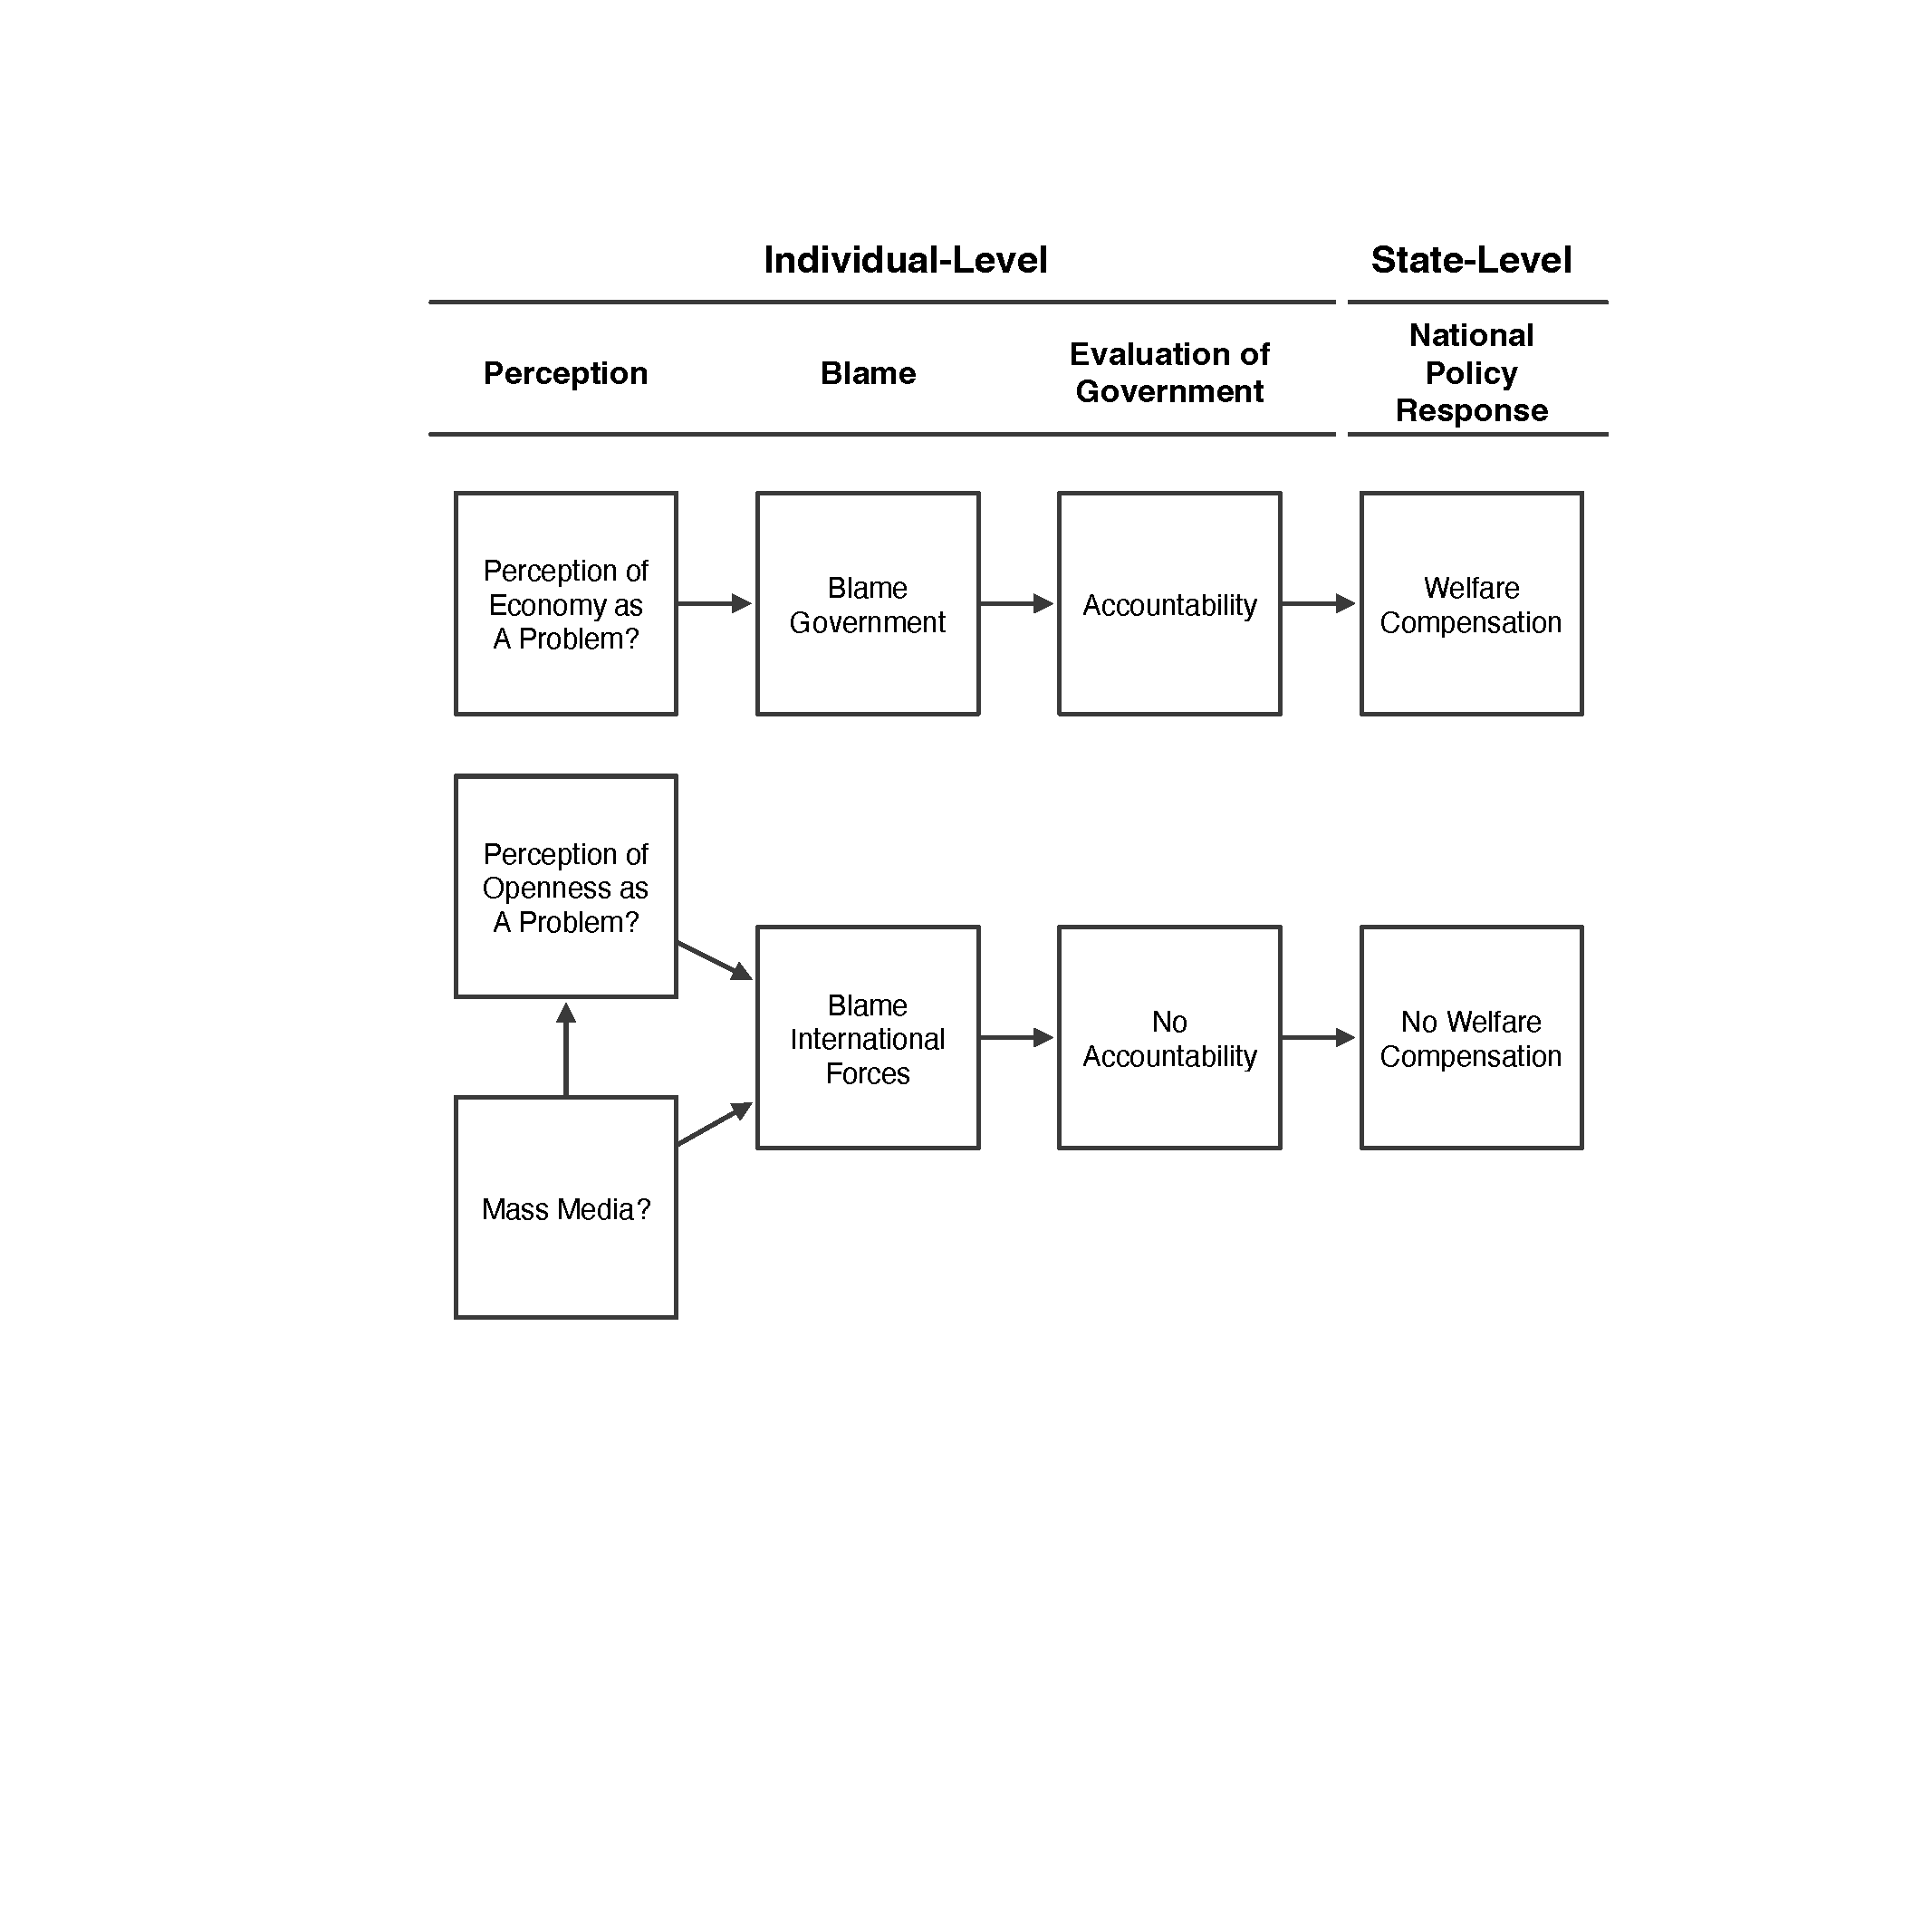
\includegraphics[scale=.45]{flowchart.pdf}}
\caption{Summary of the Hypothesized Effects of Perception and Mass Media in Domestic Responses to Economic Liberalization}
\end{figure}
\par\end{center}


\section{{\normalsize{Data and Method}}}

Given the individual-level and state-level implications of the theory,
data is gathered from both levels of analysis.%
\footnote{Full summary statistics for both datasets can be found in Supplementary
Information.%
} The individual-level data come from a Legidoscope survey of public
opinion in France between 1992 and 1993 (\citealt{Chrique:1993us}).
The survey asks respondents several questions tapping blame attribution,
media exposure, and political mobilization.%
\footnote{See Supplementary Information for the text of the survey questions. %
} Respondents are asked to identify their main source of information
from among the following: friends, family, opinion leaders, and mass
media. Respondents are also asked to identify the top two problems
facing France, and whether individuals, social institutions, the government,
or international forces beyond government control are to blame for
the problem.%
\footnote{Respondents were asked to identify national problems in an open-ended
fashion; their answers were then coded by the interviewer and into
the general problem types listed here. To create the binary variable
which measures whether the respondent sees some aspect of international
economic openness as a top problem, I coded respondents as 1 if they
identified one of the following issues as one of the ``second most
important problems'': ``Int’l economic competition,'' ``EC-92,
economic integration,'' ``Foreign trade,'' ``Ratification of Maastricht,''
and ``Maastricht Treaty.'' All other respondents were coded as 0
for the variable $Openness\: Problem$.%
} Finally, respondents are asked about their satisfaction with President
Mitterrand, how well they think the government is handling the problem
identified by the respondent as a top problem, and their intention
to turnout for the March 1993 elections. There are several reasons
why French survey data from the early 1990s represents a uniquely
useful laboratory for testing the individual-level hypotheses. First,
while other surveys gauge perceptions of responsibility on many issues,
and many other surveys gauge media exposure, this is the only survey
known to the author which effectively gauges both perceptions of responsbility
for issues of economic openness and media exposure. Second, although
the survey data is limited to France and therefore limits our ability
to generalize to other countries, France is a hard case for testing
the hypotheses, and so evidence for the hypotheses would suggest such
a process is likely to occur in other countries as well. First, the
survey takes place around the time of the Maastricht Treaty, a time
when the problems of economic openness are highly policy-related.
If media diffuses blame away from governments and onto international
forces in France in the early 1990s, mass media is even more likely
to do the same in situations where problems of economic openness are
less related to high-visibility policy decisions. Additionally, France
has relatively high rates of political engagement, and a statist,
egalitarian political culture in which elite opinion claims more control
over globalization than in countries such as Italy or the United Kingdom
(\citealt[159]{Hay:2011dh}). Thus, evidence that mass media leads
French citizens near the time of the Maastricht Treaty to blame international
forces rather than their government suggests that such a relationship
is even more likely in countries where globalization is more widely
seen as ineluctable. Although ideally the hypotheses could be tested
in multiple countries at once, this particular survey offers an ideal
opportunity to test the hypotheses under conditions relatively favorable
to generalization.

To test the direct and indirect effects of mass media on blame (Hypothesis
1), I estimate two logistic regression models. The first estimates
the probability a respondent will blame international forces as a
function of mass media exposure and a vector of control variables
including controls for the nature of the problem. The equation is

\begin{equation}
Blame_{i}=\alpha+\beta_{1}ProblemArea_{i}+\beta_{2}Openness\: Problem_{i}+\beta_{3}Media_{i}+\beta_{4}Controls_{i}+e_{i}
\end{equation}


\noindent where $Blame$ is a binary variable taking a value of 1
for respondents who blame international forces and 0 for respondents
who blame the government for whichever national problem they have
identified.%
\footnote{Because of space constraints and for ease of interpretation in light
of the hypotheses under consideration, I consider here only the difference
between blaming the government and blaming international forces, omitting
respondents who placed the blame on ``society'' or ``people like
you and me.'' However, the results obtained here are robust to alternative
specifications in which the dependent variable takes a value of 1
for respondents who blame international forces and 0 for respondents
who select any of the other possible targets of blame. See Supplementary
Information for full results.%
} $ProblemArea$ is a categorical variable with four levels indicating
whether the problem deals with social, economic, political, or foreign
issues;%
\footnote{In the first wave of the survey, so many respondents identified unemployment
as the top problem facing France that a question was added to measure
what respondents identified as the ``second most important problem
facing France today.'' All the analyses here, including the variables
measuring blame attributions and evaluations of government handling,
refer to this second most important problem.%
} $Openness\: Problem$ is a binary variable I constructed to take
a value of 1 for respondents who identified a problem specifically
related to economic openness and 0 otherwise. If the mass media have
an independent effect on diffusing blame away from government policymakers
and toward international forces, then we would expect $\beta_{3}$
to be positive and significant.

Then, to assess the indirect effect of mass media on blame as its
channeled through perceptions of economic openness, I estimate a logistic
regression modeling the probability of perceiving openness as a top
problem as a function of mass media exposure and a vector of control
variables:

\begin{equation}
Openness\: Problem_{i}=\alpha+\beta_{1}ProblemArea_{i}+\beta_{2}Media_{i}+\beta_{3}Controls_{i}+e_{i}
\end{equation}


where the main variables of interest are the same as in Equation 1
except that here the dependent variable is the binary variable capturing
whether openness is perceived as a top problem. If mass media affect
blame attributions indirectly by making individuals more aware of
international economic forces, which in turn would shift their blame
toward international forces, then $\beta_{2}$ should be positive
and significant.

To test Hypothesis 2 regarding the effect of blame attributions on
evaluations of the government, I estimate a linear regression modeling
how individuals evaluate the government's handling of the problem
they identified as one of the most important facing the country. I
model evaluations of government handling as a function of respondents'
blame attributions and a vector of control variables. The equation
is

\begin{equation}
GovHandling_{i}=\alpha+\beta_{1}ProblemArea_{i}+\beta_{2}OpennessProblem_{i}+\beta_{3}Blame_{i}+\beta_{4}Controls_{i}+e_{i}
\end{equation}


\begin{doublespace}
\noindent where $ $$GovHandling_{i}$ measures, on a scale from 1
to 4, how the \emph{i}th respondent evaluates the government's handling
of the top problem they identified. The theory predicts that for a
particular problem such as the domestic costs of economic openness,
blaming international forces rather than the government will make
individuals less likely to hold governments accountable for that problem.
If this is the case, then individuals who think a problem is caused
by forces outside of the government's purview should be less critical
of the government's handling of that problem. In this case, then,
the theoretical expectation is that $ $$\beta_{3}$ will be positive
and significant, reflecting that blaming international forces for
a problem leads individuals to view the government's handling of that
problem more favorably than if they blamed the government for the
problem.
\end{doublespace}

To test Hypothesis 3, all state-level economic data are gathered from
the World Bank's World Development Indicators (\citealt{WorldDevelopmentIn:2012wl}),
unless otherwise noted. Media penetration rates come from the World
Development Indicators and Arthur Banks' Cross-National Time-Series
Data Archive (\citealt{CrossNationalTime:td,WorldDevelopmentIn:2012wl}).%
\footnote{Summary statistics can be found in Supplementary Information.%
} The variable \emph{Democracy }is the conventional measure using the
20-point scale from Polity IV (\citealt{PolityIVProjectP:2011uq}),
reflecting a country's score for democratic institutions minus its
score for autocratic institutions. Most models have around 130 countries
with an average of roughly 8 observations per country. To test whether
mass media affects domestic compensation for globalization at the
state level, I fit several variants of the pooled cross-sectional,
time-series regression equation:

\begin{equation}
Spending_{it}=\alpha+\beta_{1}Trade_{it-1}+\beta_{2}MDI_{it-1}+\beta_{3}Trade_{it-1}*MDI_{it-1}+\beta_{4}Controls_{it-1}+e_{it}
\end{equation}


\noindent where the dependent variable, $Spending_{it}$, is a measure
of final government consumption expenditure for country $i$ in year
$t$. Final government consumpiton expenditure is a standard measure
of social welfare spending\emph{. Trade} indicates imports plus exports
as a percentage of GDP.\emph{ MDI} indicates an additive index of
media density measuring television, newspaper, and radios per capita
(\citealt{Camber:2013ul}). Because the theory deals with the conditioning
effects of mass media on domestic exposure to the global economy,
I am most interested in the multiplicative interaction of trade and
mass media ($Trade_{it-1}*MDI_{it-1}$) rather than the independent
marginal effects. If mass media exposure has the individual-level
effects hypothesized above, then an increasing density of mass media
technologies within a state should weaken the positive relationship
historically observed between levels of trade openness and levels
of domestic spending. In other words, the coefficient $\beta_{3}$
should be negative and significant, reflecting that the predicted
effect of trade on spending given high levels of mass media is less
than the predicted effect that trade has on spending given low levels
of mass media. In the first models testing Hypothesis 3, a battery
of controls are included to account for non-trade and non-media determinants
of government consumption expenditure. Data for testing particular
rival explanations are more limited and therefore reduce the geographic
and temporal coverage of the main economic and media data. For this
reason, I check the robustness of my models against alternative explanations
in a set of subsequent models.


\section{{\normalsize{Findings and Discussion}}}

Before analysis, all numerical independent variables were de-meaned
and divided by two standard deviations so that coefficients reflect
the expected effect of a two standard deviation increase in the variable
and are therefore roughly comparable to the coefficients for any categorical
independent variables (Gelman \citeyear{Gelman:2008gz}). The coefficient
plots in Figures 2 and 3 show mixed statistical support for Hypothesis
1 regarding the expectation that mass media diffuse blame for national
problems away from governments and toward international forces (directly
and indirectly).%
\footnote{On the utility of graphs in lieu of tables, see \citet{Kastellec:2007ha}.
Numerical model results are included in Supplementary Information.
All models were estimated with the \emph{Zelig} package in R (\citealt{ZeligEveryonesSt:2009ts}).%
} Respondents who rely on the mass media as their most important source
of information are significantly more likely to blame international
forces for what they identify as one of the nation's top problems
(a logit estimate of .35 and standard error of .12), even controlling
for perceptions of economic openness as a problem and the more general
issue area in which a respondent locates that problem. To get a better
sense of the effect size, consider probabilities. Based on 1000 simulations,
the probability of blaming international forces for a typical individual
who does not rely primarily on the mass media for information is .33.
Relying primarily on mass media increases this probability to .41
(a mean change of .08 with a standard deviation of .03).%
\footnote{``Typical'' refers to mean values on the numerical independent variables
and the reference levels for categorical variables, i.e., in this
case, a non-urban, non-university-educated, non-white-collar, non-left-party
male at the mean age and with mean levels of political interest, who
identifies the second top problem as ``Economic'' and not related
to economic openness.%
} Also as we would expect from previous research on public opinion
and voting in open economies, the perception of economic openness
as a problem also increases the probability a respondent will blame
international forces for that problem.%
\footnote{It could be the case that individuals with cosmopolitan outlooks are
more interested in mass media \emph{because} of their greater interest
in global issues, in which case mass media exposure could be endogenous
to knowledge of issues surrounding economic globalization. Although
the survey data used in this paper provide no measure of overall interest
in international affairs, the analyses below control for the best
predictors of cosmpolitanism: education, class, and general interest
in politics. Because these are the best predictors of cosmpolitanism,
it is unlikely that a partial, independent effect of mass media exposure
would be spurious due to this particular risk of endogeneity.%
} Indeed, of all the variables considered here, the perception of economic
openness as one of the nation's top problems is the strongest determinant
of whether a respondent will blame international forces for that problem
(a logit estimate of 1.1 and standard error of .14). In this case,
for a typical individual who identifies a top problem other than one
of openness the probability of blaming international forces is .41
but for the same individual who identifies a top problem related to
openness, that probability increases to .68 (a mean increase of .26
and standard deviation .03). To check the robustness of this finding,
I also estimate several models using different operationalizations
of the dependent variable.%
\footnote{Whereas Model 1 considers for simplicity the binary opposition between
blaming the government (dependent variable equal to 0) and blaming
international forces (dependent variable equal to 1), I estimated
additional models where the binary dependent variable opposes each
of these targets of blame to anyone who blames any other target. See
Supplementary Information.%
} These additional models are consistent with the evidence presented
in this section. 

\begin{figure}
\begin{centering}
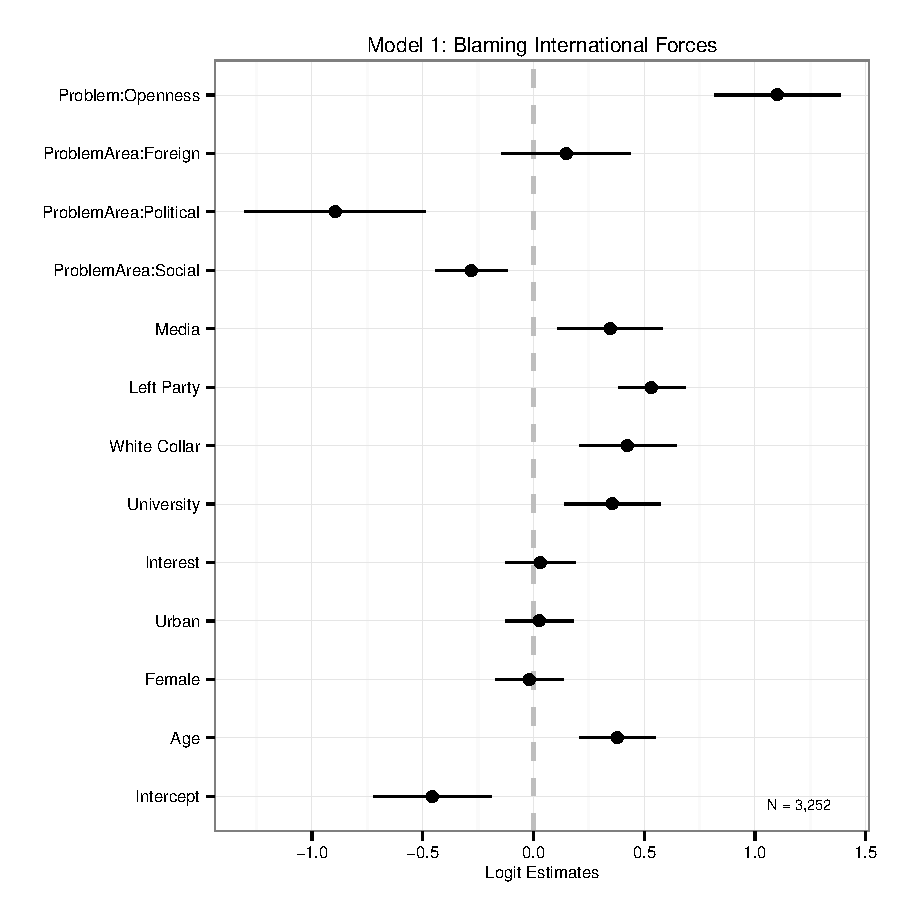
\includegraphics{model1}
\par\end{centering}

\caption{Determinants of Blaming International Forces}
\end{figure}


Model 2 considers the indirect effect of mass media on blame attributions
through their effect on perceptions of openness as a problem. Reliance
on mass media has a positive marginal effect on the perception of
openness as a problem (a logit estimate of .33 and standard error
of .17; \emph{p}=.06). For a typical individual who does not rely
primarily on mass media, the probability of perceiving an issue of
openness to be a top problem is .08; relying on mass media increases
this probability by a mean of .03 (standard deviation = .01) to .11.
Thus, the indirect effect of mass media on blaming international forces,
through its slight marginal effect on the perception of openness as
a problem, is merely .01 (.26{*}.03). The small size of this effect
and its statistical significance near the conventional cutoff of 95\%
confidence suggest only weak evidence that mass media exerts much
indirect effect on blame attributions by increasing awareness of openness
as a problem.

\begin{figure}
\begin{centering}
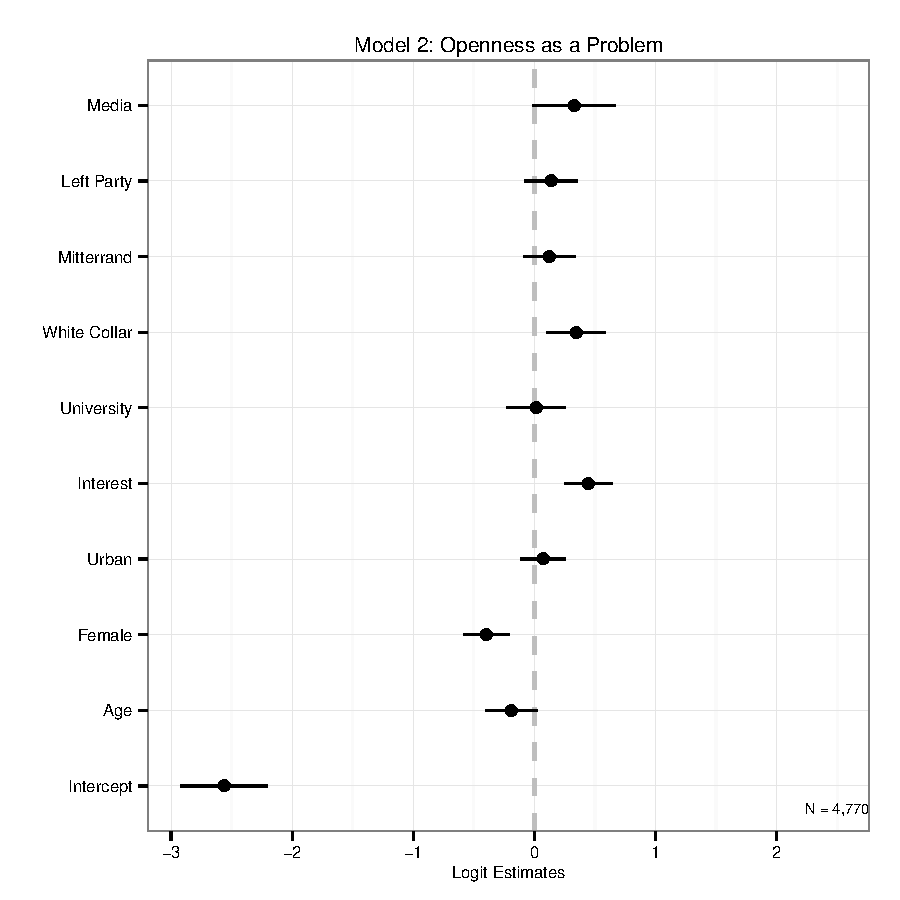
\includegraphics{model2}
\par\end{centering}

\caption{Determinants of Perceiving Openness as a Top Problem}
\end{figure}


The coefficient plot for Model 3, testing Hypothesis 2, reveals statistical
evidence for the expectation that blaming international forces, in
turn, has a positive effect on evaluations of the government \emph{(}logit
estimate = .38, standard error = .03).%
\footnote{There is reason to suppose that blame attributions could be endogenous
to evaluations of how the government is handling a problem, in the
sense that perceptions of poor or satisfactory government handling
could increase or decrease the government's perceived culpability.
First, however, it should be recalled that survey question I am using
to measure blame attributions refers specifically to the cause of
the problem. Thus, strictly speaking, evaluations of how the government
handles the problem should not affect who or what individuals identify
as the cause or source of the problem. Second, it is much harder to
believe that evaluations of government handling could drive individuals'
blame of international forces or blame of the two alternative targets
from which respondents were able to choose (individuals ``like you
and I'' or social institutions) simply because it is hard to imagine
how government handling of the problem could make any of these other
targets more or less culpable. Thus, I estimate an additional model
which has separate binary independent variables for blaming government,
international forces, or ``other'' as the baseline (see Supplementary
Information). The coefficient for blaming government is larger than
that for blaming international forces but both remain signed as expected
and significant. This alternative specification mitigates the possibility
that blaming international forces merey reflects respondents who are
less likely to blame the government. Finally, if it can be assumed
that endogeneity between evaluations of handling and blame would be
most likely among partisans, then the control for partisanship and
the two separate controls for support of President Mitterrand likely
absorb much of this endogeneity.%
} Simulating quantities of interest suggests that blaming international
forces for a top problem increases a typical individual's evaluation
of government handling by .38 (standard devation = .03), from 1.6
to 2.0 on the four-point scale of the dependent variable. These results
also hold when the dependent variable refers to satisfaction with
the President rather than government handling of a top problem. They
are also robust to an expanded operationalization of the blame variable
considering the government, international forces, and other possible
targets.%
\footnote{See Supplementary Information. %
}
\begin{figure}
\begin{centering}
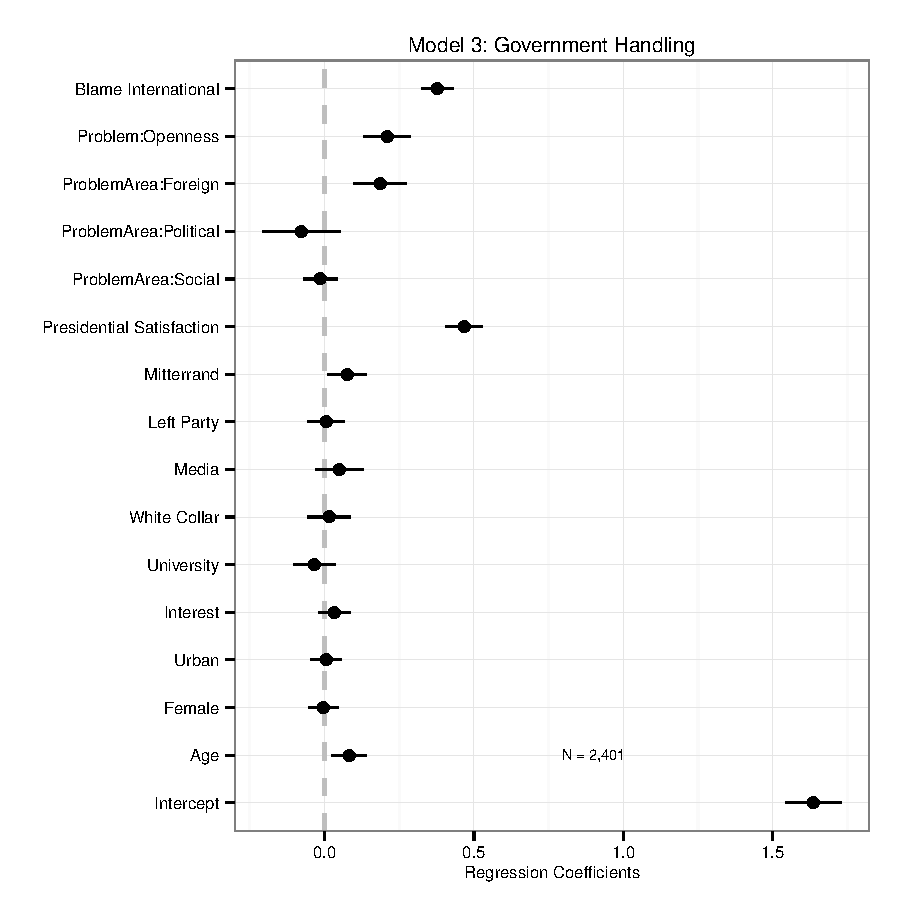
\includegraphics{model3}
\par\end{centering}

\caption{Determinants of Government Evaluations}
\end{figure}


Thus the results provide evidence consistent with each essential step
of the causal chain at the individual level, though the estimated
indirect effect of mass media on diffusing blame (through increasing
perceptions of openness as a problem) is very weak. Nonetheless, the
evidence suggests that mass media directly diffuse blame away from
governments toward international forces (increasing the probability
of blaming international forces by about 8\%) even controlling for
the general issue area in which the respondent locates a top problem
and whether it is related to openness.

Table 1 displays results from three regression models which provide
initial support for the state-level expectations regarding the effect
of mass media on the globalization-welfare relationship. Models 4
and 5 consider variable levels only, while Model 6 is an error-correction
model using first-differences (year-to-year changes) in the dependent
variable and lagged levels of the dependent variable on the right-hand
side of the equation, alongside levels and first-differences of the
key independent variables.%
\footnote{For Model 6, inclusion of a second lag of level of spending ($t-2$)
makes the covaration matrix non-invertible and therefore precludes
a unique estimation of the model. However, omitting it leads us to
reject the null hypothesis of no serial correlation in the error term
according to the Breusch-Godfrey test for panel models (p=0.026).
I therefore use $Spending_{it-3}$on the right-hand side of the equation,
which leads us to fail to reject the null hypothesis of no serial
correlation (p=.13).%
} Although a level dependent variable with a lagged level on the right-hand
side is formally equivalent to a differenced dependent variable, the
error-correction specification is useful here because it allows us
to separate short-run and long-run effects.%
\footnote{The error-correction specification is useful here for another reason.
Although government spending and media density are not quite co-integrated,
they are nearly cointegrated. In such situations, error-correction
specifications are ideal for insuring against the possibility of spurious
correlations driven by that shared integration. %
} The differenced independent variables reflect immediate, short-run
effects and the level independent variables reflect the long-run effect
after the short-run effects decay. All three models include fixed
effects for country and year to account for unobserved differences
in countries or unobserved temporal shocks in any particular year.%
\footnote{This was done using the ``within'' transformation and ``two-way''
effect option in the \emph{plm }package for R (\citealt{Croissant:2013ty}).%
} To control for the clustering of errors within countries and the
possibility of downwardly biased standard errors, I also calculate
panel-corrected standard errors following Beck and Katz (\citeyear{Beck:1995hm}).
Panel-corrected standard errors did not appreciably change the statistical
significance of any estimates reported in this paper.%
\footnote{It is common to display the panel-corrected standard errors rather
than the untransformed errors, but it is not obvious that treating
them as a default has improved our use of cross-sectional, time-series
data. On this point, see \citet{Wilson:2007kz}, with whom I take
the view that panel-corrected standard errors are only one of many
checks against difficulties common in cross-sectional, time-series
data. Fixed effects, lagged dependent variables, and dynamic specifications
are some of the other techniques stressed by those authors. Here,
I employ all of these latter techniques, and in some cases all together.%
}

In each of the three model specifications, the variable $Trade_{it-1}*MDI_{it-1}$
is negative and statistically significant, suggesting that media density
decreases the association between levels of trade and subsequent levels
of government consumption expenditure. The coefficient of -.97 for
$Trade_{it-1}*MDI_{it-1}$ in Model 4 suggests that, on average, a
two standard deviation increase in media density (109.3 points) in
the long-run decreases the estimated effect that a two standard deviation
increase in trade openness (85.2\% of GDP) would have on government
spending by .97\% of GDP. Model 6 estimates that this negative conditioning
effect of media density is as little as .61\% of GDP. Moving from
the minimum density of media (0) to the maximum in the sample (313.3)
is associated, on average, with a decrease of as much as 2.78\%, and
as little as 1.8\%, in the expected effect of an 85\% increase in
trade openness on government spending as a share of GDP. Although
the estimated effect appears relatively slight, it should be kept
in mind that the mean level of government consumption expenditure
in the sample is only 15.7\% of GDP. Thus, for a country that begins
with no mass media and becomes as fully penetrated as the most penetrated
(the United States in 1986), the roughly 1-3\% of GDP by which we
would expect the country to reduce its compensatory public spending
in the long-run for an 85\% increase in trade openness is a substantial
portion of what a typical country spends.

Models 5 and 6 also tests the conditioning effect of media density
against the conditioning effects of democracy on the trade-welfare
relationship, which previous research has found to increase the redistributive
responsiveness of domestic welfare spending to international trade
(\citealt{Adsera:2002vt}). The results here suggest that media density
has a robust conditioning effect on the relationship between trade
and spending, while the interaction found by Adserà and Boix no longer
appears statistically distinguishable from zero.

To check for the possibility that the above models are spuriously
driven by some different but unobserved process distinct from the
effects of mass media, I gather additional data to test my state-level
argument against a series of rival explanations. Specifically, it
is argued that left parties and union density are aspects of the domestic
institutional environment which lead to more redistributive responses
to economic liberalization (\citealt[674]{Garrett:1995tj}); that
electoral systems defined by proportional representation are more
redistributive than majoritarian systems (\citealt{Iversen:2006wd});
and that the degree of unitarism or government centralization affects
welfare spending (\citealt[72]{Crepaz:1998vj}). Finally, of particular
interest in the literature relating economic globalization to the
politics of welfare is the argument of Iversen (\citeyear{Iversen:2001vr})
and Iversen and Cusack (\citeyear{Iversen:2000ch}) that deindustrialization
rather than globalization has driven the expansion of welfare spending
since the 1960s.

\def\sym#1{\ifmmode^{#1}\else\(^{#1}\)\fi}
\begin{table}[htbp]
\caption {Determinants of Government Consumption Expenditure} \label{tab:title} 
\centering
\footnotesize
\begin{tabular}{l*{3}{c}}
\hline\hline
  &\multicolumn{1}{c}{spending.wb} &\multicolumn{1}{c}{spending.wb} &\multicolumn{1}{c}{diff(spending.wb)} \\
\hline
lag(trade.wb, 1) 		&0.144 		&0.147 		&0.38\sym{*}\\
  		&(0.213) 		&(0.213) 		&(0.222) \\
lag(mdi, 1) 		&-0.157 		&-0.114 		&0.612\sym{*} \\
  		&(0.402) 		&(0.403) 		&(0.318) \\
lag(polity2, 1) 		&0.025 		&-0.03 		& \\
  		&(0.152) 		&(0.157) 		& \\
lag(gdpcap.wb, 1) 		&0.615\sym{***} 		&0.608\sym{***} 		& \\
  		&(0.189) 		&(0.189) 		& \\
lag(dependency.wb, 1) 		&-0.218 		&-0.235 		& \\
  		&(0.231) 		&(0.232) 		& \\
lag(land.wb, 1) 		&13.921 		&20.356 		& \\
  		&(191.648) 		&(191.676) 		& \\
lag(spending.wb, 1) 		&0.717\sym{***} 		&0.716\sym{***} 		&-0.164\sym{***} \\
  		&(0.016) 		&(0.016) 		&(0.01) \\
lag(spending.wb, 2) 		&0.11\sym{***} 		&0.111\sym{***} 		& \\
  		&(0.016) 		&(0.016) 		& \\
lag(trade.wb, 1):lag(mdi, 1) 		&-0.97\sym{***} 		&-0.883\sym{***} 		&-0.611\sym{*} \\
  		&(0.32) 		&(0.325) 		&(0.317) \\
lag(diff(trade.wb)):lag(diff(mdi)) 		& 		& 		&8.139 \\
  		& 		& 		&(15.681) \\
lag(trade.wb, 1):lag(polity2, 1) 		& 		&-0.428 		&-0.434 \\
  		& 		&(0.303) 		&(0.294) \\
lag(diff(trade.wb)):lag(diff(polity2)) 		& 		& 		&-3.557\sym{*} \\
  		& 		& 		&(1.963) \\
lag(diff(trade.wb), 1) 		& 		& 		&-0.946\sym{**} \\
  		& 		& 		&(0.388) \\
lag(diff(mdi), 1) 		& 		& 		&0.562 \\
  		& 		& 		&(1.716) \\
lag(diff(polity2), 1) 		& 		& 		&-0.056 \\
  		& 		& 		&(0.284) \\
lag(diff(gdpcap.wb), 1) 		& 		& 		&0.668 \\
  		& 		& 		&(0.723) \\
lag(diff(dependency.wb), 1) 		& 		& 		&2.4 \\
  		& 		& 		&(1.794) \\
lag(diff(spending.wb), 1) 		& 		& 		&-0.104\sym{***} \\
  		& 		& 		&(0.016) \\
\hline
$R^2$ 		&0.672 		&0.672 		&0.104 \\
$adj.R^2$ 		&0.638 		&0.638 		&0.098 \\
$N$ 		&\multicolumn{1}{c}{3911} 		&\multicolumn{1}{c}{3911} 		&\multicolumn{1}{c}{3914} \\
\hline\hline
\multicolumn{4}{l}{\footnotesize Standard errors in parentheses}\\
\multicolumn{4}{l}{\footnotesize $^{*}$ (p $\le$ 0.1), $^{**}$ (p $\le$ 0.05), $^{***}$ (p $\le$ 0.01)}\\
\end{tabular}
\end{table}


In Table 2, I re-estimate the error-correction model (as in Model
6 of Table 1) controlling for each of the rival explanations above.%
\footnote{See Supporting Information for more information on variable descriptions
and sources.%
} The interaction of trade levels and media density levels is robust
to the inclusion of each potentially confounding variable, suggesting
that the conditioning effect of media density on the trade-spending
relationship is not a spurious correlation due to an omitted variable.
In an additional model not displayed for lack of space, I included
the terms $Trade{}_{it-1}*GDPPerCapita{}_{it-1}$ and $\Delta Trade{}_{it-1}*\Delta GDPPerCapita{}_{it-1}$
on the right-hand side of the equation in the fashion of the models
in Table 2; neither coefficient is statistically significant and the
main independent variable of interest, $Trade_{it-1}*MDI_{it-1}$,
remains signed as expected and statistically significant ($\beta$=-1.56,
standard error=.000, panel-corrected standard error=.005).

\def\sym#1{\ifmmode^{#1}\else\(^{#1}\)\fi}
\begin{table}[htbp]
\footnotesize
\centering
\caption{Rival Explanations: Electoral System, Centralization, Left Party Seats, Union Density, and De-Industrialization}
\begin{tabular}{l*{5}{c}}
\hline\hline
  &\multicolumn{1}{c}{(1)} &\multicolumn{1}{c}{(2)} &\multicolumn{1}{c}{(3)} &\multicolumn{1}{c}{(4)} &\multicolumn{1}{c}{(5)} \\
\hline
lag(diff(trade.wb), 1) 		&-0.668 		&-0.429 		&-2.431\sym{**} 		&-1.362 		&-1.345\sym{***} \\
  		&(0.458) 		&(0.467) 		&(1.055) 		&(0.879) 		&(0.481) \\
lag(mdi, 1) 		&0.045 		&-0.014 		&-0.278 		&-0.589\sym{**} 		&-0.047 \\
  		&(0.416) 		&(0.416) 		&(0.262) 		&(0.242) 		&(0.677) \\
lag(diff(mdi), 1) 		&0.814 		&0.743 		&2.258\sym{***} 		&2.839\sym{***} 		&-0.919 \\
  		&(1.743) 		&(1.741) 		&(0.775) 		&(0.821) 		&(2.253) \\
lag(gdpcap.wb, 1) 		&0.472\sym{**} 		&0.509\sym{***} 		&0.556\sym{***} 		&0.427\sym{***} 		&0.833\sym{***} \\
  		&(0.187) 		&(0.187) 		&(0.137) 		&(0.117) 		&(0.285) \\
lag(spending.wb, 1) 		&-0.233\sym{***} 		&-0.234\sym{***} 		&-0.071\sym{***} 		&-0.075\sym{***} 		&-0.247\sym{***} \\
  		&(0.014) 		&(0.014) 		&(0.018) 		&(0.015) 		&(0.013) \\
lag(trade.wb, 1):lag(mdi, 1) 		&-0.662\sym{*} 		&-0.641\sym{**} 		&-0.891\sym{**} 		&-1.184\sym{***} 		&-1.919\sym{***} \\
  		&(0.342) 		&(0.324) 		&(0.354) 		&(0.314) 		&(0.542) \\
lag(diff(trade.wb), 1):lag(diff(mdi), 1) 		&5.072 		&4.268 		&-39.462 		&-41.014 		&41.667\sym{*} \\
  		&(18.142) 		&(18.194) 		&(25.394) 		&(25.531) 		&(25.254) \\
lag(pr, 1) 		&0.476 		& 		& 		& 		& \\
  		&(0.359) 		& 		& 		& 		& \\
lag(trade.wb, 1):lag(pr, 1) 		&0.296 		& 		& 		& 		& \\
  		&(0.334) 		& 		& 		& 		& \\
lag(diff(trade.wb), 1):lag(diff(pr), 1) 		&-11.343\sym{***} 		& 		& 		& 		& \\
  		&(3.858) 		& 		& 		& 		& \\
lag(unitarism, 1) 		& 		&-0.695 		& 		& 		& \\
  		& 		&(0.681) 		& 		& 		& \\
lag(trade.wb, 1):lag(unitarism, 1) 		& 		&0.651 		& 		& 		& \\
  		& 		&(0.536) 		& 		& 		& \\
lag(diff(trade.wb), 1):lag(diff(unitarism), 1) 		& 		&-12.632\sym{*} 		& 		& 		& \\
  		& 		&(6.579) 		& 		& 		& \\
lag(netden, 1) 		& 		& 		&-0.086 		& 		& \\
  		& 		& 		&(0.167) 		& 		& \\
lag(trade.wb, 1):lag(netden, 1) 		& 		& 		&-0.8\sym{**} 		& 		& \\
  		& 		& 		&(0.393) 		& 		& \\
lag(diff(trade.wb), 1):lag(diff(netden), 1) 		& 		& 		&-14.819 		& 		& \\
  		& 		& 		&(21.369) 		& 		& \\
lag(lefts, 1) 		& 		& 		& 		&0.208\sym{*} 		& \\
  		& 		& 		& 		&(0.125) 		& \\
lag(trade.wb, 1):lag(lefts, 1) 		& 		& 		& 		&0.441 		& \\
  		& 		& 		& 		&(0.343) 		& \\
lag(diff(trade.wb), 1):lag(diff(lefts), 1) 		& 		& 		& 		&-2.568 		& \\
  		& 		& 		& 		&(4.755) 		& \\
lag(industry.wb, 1) 		& 		& 		& 		& 		&0.06 \\
  		& 		& 		& 		& 		&(0.253) \\
lag(diff(industry.wb), 1) 		& 		& 		& 		& 		&-0.862\sym{*} \\
  		& 		& 		& 		& 		&(0.517) \\
lag(mdi, 1):lag(industry.wb, 1) 		& 		& 		& 		& 		&0.495 \\
  		& 		& 		& 		& 		&(0.56) \\
lag(diff(mdi), 1):lag(diff(industry.wb), 1) 		& 		& 		& 		& 		&56.869\sym{**} \\
  		& 		& 		& 		& 		&(25.815) \\
\hline
$R^2$ 		&0.125 		&0.123 		&0.194 		&0.147 		&0.144 \\
$adj.R^2$ 		&0.115 		&0.114 		&0.17 		&0.131 		&0.134 \\
$N$ 		&\multicolumn{1}{c}{2224} 		&\multicolumn{1}{c}{2224} 		&\multicolumn{1}{c}{544} 		&\multicolumn{1}{c}{673} 		&\multicolumn{1}{c}{2736} \\
\hline\hline
\multicolumn{6}{l}{\footnotesize Standard errors in parentheses. For space constraints, estimates for land, dependency rates, levels of trade}\\
\multicolumn{6}{l}{\footnotesize and democracy are included but not displayed (all were indistinguishable from zero at 95\% confidence).}\\
\multicolumn{6}{l}{\footnotesize $^{*}$ (p $\le$ 0.1), $^{**}$ (p $\le$ 0.05), $^{***}$ (p $\le$ 0.01)}\\
\end{tabular}
\end{table}


Several additional robustness checks were conducted. With panel data,
Nickell bias can lead to rejecting a true null hypothesis when the
number of units is large relative to the time period \citep{Gaibulloev:2014eg}.
Given that the present panel contains a relatively large number of
countries with a sampling period of more than 30 years (the period
beyond which Nickell bias becomes ignorable), I re-estimate the models
in Table 2 on only those countries with complete data for the 38 years
between 1961 and 1999. Table 12 in Supplementary Information shows
the results, substantially the same as the those reported here. I
also checked sensitivity to lag specification for $Trade_{it-1}*MDI_{it-1}$
estimating the models in Table 1 using $Trade_{it}*MDI_{it}$ as the
independent variable instead. The coefficients and standard errors
are not substantially changed (see Table 13 in Supplementary Information).
Thefore the state-level models provide additional, robust evidence
that mass media shape perceptions and blame attributions around economic
globalization in a way that weakens the compensatory responsiveness
of welfare spending.


\section{{\normalsize{Conclusion}}}

This study has presented individual- and state-level evidence that
mass media functions as a political institution which conditions the
domestic politics of economic globalization. Because the dominant
social construction of economic globalization is that of an external
constraint imposed on policymakers by impersonal and international
forces, by amplifying this construction mass media decrease the accountability
of national economic policymakers who pursue liberalization. Survey
evidence from France shows that individuals most reliant on mass media
are less likely to blame top national problems on incumbent governments,
and more likely to blame international forces, for indirect and direct
reasons. Mass media \emph{indirectly} deflects blame away from incumbent
governments and toward international forces by making individuals
more aware of economic openness as a political issue, but it also
\emph{directly} decreases individuals' propensities to blame incumbents
relative to international forces (controlling for the awareness effect),
most likely due to the responsbility-diffusing framing effects previously
found in mass media studies. In turn, individuals who blame international
forces rather than the government evaluate the government more favorably.
Cross-sectional, time-series data reveal that mass media is associated
with a decrease in the relationship between economic openness and
welfare-state spending, providing further evidence that mass media
diffuses the domestic political pressure against liberalization that
has historically elicited welfare-state compensation for aggrieved
domestic groups. The state-level evidence is consistent with the individual-level
evidence that mass media shifts blame attributions away from governments
and toward international forces, which weakens the strategic pressure
on national economic policymakers to provide welfare-state compensation
to harmed domestic groups.

The limitations of this study also point to avenues for future research
on the attitudinal and behavioral mechanisms shaping the domestic
politics of economic globalization. While I considered many dominant
rival hypotheses through the use of statistical control variables
and the inclusion of alternative interaction terms, this article could
not engage with all possible factors that may plausibly condition
the relationships posited by the three hypotheses presented. Thus,
future research must investigate the sensitivity and conditionality
of the general findings presented here. For instance, it seems likely
that political partisanship might condition the relationship between
media exposure and blame attributions, and/or the relationship between
blame attributions and evaluations of government. Thus, rather than
simply controlling for partisanship as above, future research might
investigate whether these relationships are dampened or amplified
under different conditions of citizen and government partisanship.
Additionally, for the state-level findings, future research might
investigate whether the conditioning effect of media on the globalization-welfare
nexus is not itself conditional on region, national government partisanship,
or various factors related to the national media environment (such
as media concentration, ownership, etc.).

The findings have several implications for the study of international
and comparative politics and for the prospects of democracy in a globalized
world. First, the results provide some of the first evidence that
mass media can be understood as a political institution that conditions
the domestic politics of the global economy, thus placing on the agenda
a source of cross-national and temporal variation typically omitted
from previous analyses of comparative and international political
economy. As such, they contribute to current research agendas seeking
more finely-tuned political accounts of the domestic effects of globalization
(\citealt[341]{Kayser:2007iga}) and a better understanding of public
opinion and voting behavior in the context of economic openness (\citealt{Hellwig:2008ia,Hellwig:2008cj}).
Specifically, the article suggests that mass media is an independent
cause of voters discounting their evaluations of policymakers (by
increasing the probability they will identify economic openness as
a top problem, but also by directly diffusing blame attributions toward
international forces \emph{even holding constant the types of problems
they perceive to be most important}). The findings should be of particular
interest to scholars seeking to develop more rigorous micro-foundations
for the relationship between economic openness and welfare states
(\citealt{Hays:2005vo,Walter:2010ky}). Second, the state-level findings
in particular have an important substantive implication, for they
suggest that the omission of mass media in previous studies may have
led to biased conclusions which over-estimate the egalitarian responsiveness
of welfare states in the globalization-welfare nexus. The evidence
suggests that from the standpoint of democratic values, mass media
can have subtle but perverse effects on the distributive politics
of open economies, disempowering domestic groups from holding national
policymakers accountable for the unevenly distributed costs of globalization.

\pagebreak{}

\bibliographystyle{apsr2006}
\bibliography{bib}


\pagebreak{}
\end{document}
